% Options for packages loaded elsewhere
\PassOptionsToPackage{unicode}{hyperref}
\PassOptionsToPackage{hyphens}{url}
\PassOptionsToPackage{dvipsnames,svgnames,x11names}{xcolor}
%
\documentclass[
  ignorenonframetext,
]{beamer}
\usepackage{pgfpages}
\setbeamertemplate{caption}[numbered]
\setbeamertemplate{caption label separator}{: }
\setbeamercolor{caption name}{fg=normal text.fg}
\beamertemplatenavigationsymbolsempty
% Prevent slide breaks in the middle of a paragraph
\widowpenalties 1 10000
\raggedbottom
\setbeamertemplate{part page}{
  \centering
  \begin{beamercolorbox}[sep=16pt,center]{part title}
    \usebeamerfont{part title}\insertpart\par
  \end{beamercolorbox}
}
\setbeamertemplate{section page}{
  \centering
  \begin{beamercolorbox}[sep=12pt,center]{part title}
    \usebeamerfont{section title}\insertsection\par
  \end{beamercolorbox}
}
\setbeamertemplate{subsection page}{
  \centering
  \begin{beamercolorbox}[sep=8pt,center]{part title}
    \usebeamerfont{subsection title}\insertsubsection\par
  \end{beamercolorbox}
}
\AtBeginPart{
  \frame{\partpage}
}
\AtBeginSection{
  \ifbibliography
  \else
    \frame{\sectionpage}
  \fi
}
\AtBeginSubsection{
  \frame{\subsectionpage}
}

\usepackage{amsmath,amssymb}
\usepackage{iftex}
\ifPDFTeX
  \usepackage[T1]{fontenc}
  \usepackage[utf8]{inputenc}
  \usepackage{textcomp} % provide euro and other symbols
\else % if luatex or xetex
  \usepackage{unicode-math}
  \defaultfontfeatures{Scale=MatchLowercase}
  \defaultfontfeatures[\rmfamily]{Ligatures=TeX,Scale=1}
\fi
\usepackage{lmodern}
\usetheme[]{metropolis}
\ifPDFTeX\else  
    % xetex/luatex font selection
\fi
% Use upquote if available, for straight quotes in verbatim environments
\IfFileExists{upquote.sty}{\usepackage{upquote}}{}
\IfFileExists{microtype.sty}{% use microtype if available
  \usepackage[]{microtype}
  \UseMicrotypeSet[protrusion]{basicmath} % disable protrusion for tt fonts
}{}
\makeatletter
\@ifundefined{KOMAClassName}{% if non-KOMA class
  \IfFileExists{parskip.sty}{%
    \usepackage{parskip}
  }{% else
    \setlength{\parindent}{0pt}
    \setlength{\parskip}{6pt plus 2pt minus 1pt}}
}{% if KOMA class
  \KOMAoptions{parskip=half}}
\makeatother
\usepackage{xcolor}
\newif\ifbibliography
\setlength{\emergencystretch}{3em} % prevent overfull lines
\setcounter{secnumdepth}{-\maxdimen} % remove section numbering


\providecommand{\tightlist}{%
  \setlength{\itemsep}{0pt}\setlength{\parskip}{0pt}}\usepackage{longtable,booktabs,array}
\usepackage{calc} % for calculating minipage widths
\usepackage{caption}
% Make caption package work with longtable
\makeatletter
\def\fnum@table{\tablename~\thetable}
\makeatother
\usepackage{graphicx}
\makeatletter
\def\maxwidth{\ifdim\Gin@nat@width>\linewidth\linewidth\else\Gin@nat@width\fi}
\def\maxheight{\ifdim\Gin@nat@height>\textheight\textheight\else\Gin@nat@height\fi}
\makeatother
% Scale images if necessary, so that they will not overflow the page
% margins by default, and it is still possible to overwrite the defaults
% using explicit options in \includegraphics[width, height, ...]{}
\setkeys{Gin}{width=\maxwidth,height=\maxheight,keepaspectratio}
% Set default figure placement to htbp
\makeatletter
\def\fps@figure{htbp}
\makeatother

\definecolor{TAMUMaroon}{HTML}{500000}
\setbeamercolor{palette primary}{bg=TAMUMaroon,fg=white}
\makeatletter
\@ifpackageloaded{caption}{}{\usepackage{caption}}
\AtBeginDocument{%
\ifdefined\contentsname
  \renewcommand*\contentsname{Table of contents}
\else
  \newcommand\contentsname{Table of contents}
\fi
\ifdefined\listfigurename
  \renewcommand*\listfigurename{List of Figures}
\else
  \newcommand\listfigurename{List of Figures}
\fi
\ifdefined\listtablename
  \renewcommand*\listtablename{List of Tables}
\else
  \newcommand\listtablename{List of Tables}
\fi
\ifdefined\figurename
  \renewcommand*\figurename{Figure}
\else
  \newcommand\figurename{Figure}
\fi
\ifdefined\tablename
  \renewcommand*\tablename{Table}
\else
  \newcommand\tablename{Table}
\fi
}
\@ifpackageloaded{float}{}{\usepackage{float}}
\floatstyle{ruled}
\@ifundefined{c@chapter}{\newfloat{codelisting}{h}{lop}}{\newfloat{codelisting}{h}{lop}[chapter]}
\floatname{codelisting}{Listing}
\newcommand*\listoflistings{\listof{codelisting}{List of Listings}}
\makeatother
\makeatletter
\makeatother
\makeatletter
\@ifpackageloaded{caption}{}{\usepackage{caption}}
\@ifpackageloaded{subcaption}{}{\usepackage{subcaption}}
\makeatother
\ifLuaTeX
  \usepackage{selnolig}  % disable illegal ligatures
\fi
\usepackage{bookmark}

\IfFileExists{xurl.sty}{\usepackage{xurl}}{} % add URL line breaks if available
\urlstyle{same} % disable monospaced font for URLs
\hypersetup{
  pdftitle={Spatial Modeling of Cardiovascular Disease Incidence Positively Associated with PM2.5},
  pdfauthor={Shombit Roy, Christina Kim, Johan Booc},
  colorlinks=true,
  linkcolor={blue},
  filecolor={Maroon},
  citecolor={Blue},
  urlcolor={Blue},
  pdfcreator={LaTeX via pandoc}}

\title{Spatial Modeling of Cardiovascular Disease Incidence Positively
Associated with PM2.5}
\author{Shombit Roy, Christina Kim, Johan Booc}
\date{2024-04-27}

\begin{document}
\frame{\titlepage}

\section{Introduction}\label{introduction}

\section{Literature Review Section}\label{literature-review-section}

\begin{frame}{Literature Review}
\phantomsection\label{literature-review}
\begin{itemize}
\item
  Statistical regression + spatial models have been growing in
  popularity to analyze the distribution and factors of cardiovascular
  disease~
\item
  A good amount of other studies focus on socioeconomic covariates and
  their impact on cardiovascular disease mortality rates however, our
  study takes into account PM2.5 concentrations~
\item
  By analyzing the spatial distribution of our covariates, we can
  provide risk estimates for the year 2015
\end{itemize}
\end{frame}

\begin{frame}{Literature Review}
\phantomsection\label{literature-review-1}
\begin{itemize}
\item
  The geographically weighted model builds on the weighted least squares
  method and considers coefficients for each spatial unit for
  estimation~
\item
  We are interested in seeing the values that carry more weight because
  they carry a greater amount of influence
\end{itemize}
\end{frame}

\begin{frame}{Literature Review}
\phantomsection\label{literature-review-2}
\begin{itemize}
\item
  The ordinary least squares method generates global regression
  coefficients however it's prone to hidden spatial variability~
\item
  We use the GWR model to test and verify our results to be
  statistically significant, treating the OLS model as the null~
\item
  The GWR model minimizes errors between the actual and predicted
  values, which helps health practitioners narrow down the areas for
  improvement
\end{itemize}
\end{frame}

\section{Methods Section}\label{methods-section}

\begin{frame}{Methods}
\phantomsection\label{methods}
\begin{itemize}
\item
  Medicare claims, racial/geographic data from the Census and TIGER
  Bureau, median income from Census API, air quality from NASA PM2.5
  data, and unemployment rates loaded from CDC.
\item
  Grouped data by year, county, and coordinates for 2015; cleaned by
  removing entries with empty geometries and incomplete data,~ excluding
  Alaska and Hawaii, which led to Nantucket County being removed from
  the dataset
\end{itemize}
\end{frame}

\begin{frame}{Methods}
\phantomsection\label{methods-1}
\begin{itemize}
\item
  Transformed integrated data into a format suitable for Geographical
  Weighted Regression (GWR) by calculating centroids of the
  multi-polygon geometries to provide a single point to get precise
  location-based assessments.~
\item
  Cross-validation was utilized to estimate the optimal fixed bandwidth
  for the GWR model
\item
  The Gaussian kernel was chosen for its smoothness
\end{itemize}
\end{frame}

\begin{frame}{Model}
\phantomsection\label{model}
\(y = \beta_0*\%White +\beta_1* \%Black + \beta_2 *\%Hispanic + \beta_3 *\%Asian + \beta_4 *PM2.5 + \beta_5 * Median Income + \beta_6 * \%Unemployed\)
\end{frame}

\begin{frame}{Methods}
\phantomsection\label{methods-2}
\begin{itemize}
\item
  Geographic plots visualize the spatial distribution of CVD death rates
  across different US counties
\item
  Significance of various socioeconomic, environmental, and demographic
  factors on CVD death rates is analyzed regionally.
\end{itemize}
\end{frame}

\begin{frame}{Simulation}
\phantomsection\label{simulation}
\begin{itemize}
\item
  Simulated data is used with a piecewise function dividing the
  geographical space into quadrants, each assigned different
  coefficients to model spatial heterogeneity
\item
  A spatial autocorrelation test (Moran's I) is performed on the
  residuals of the GWR model
\end{itemize}
\end{frame}

\section{Results Section}\label{results-section}

\begin{frame}{Results}
\phantomsection\label{results}
\begin{itemize}
\item
  The global regression model:

  \begin{itemize}
  \item
    Shows all predictors as statistically significant.
  \item
    Does not consider spatial correlation, potentially missing local
    variations.
  \item
    Residual analysis reveals spatial patterns, with clusters of higher
    and lower residuals indicating missed spatial variation.
  \end{itemize}
\end{itemize}

\begin{itemize}
\item
  The GWR model:

  \begin{itemize}
  \item
    Incorporates spatial variation, addressing a critical aspect of the
    data.
  \item
    Provides a more nuanced and realistic interpretation of how various
    factors affect death rates across different regions.
  \end{itemize}
\end{itemize}
\end{frame}

\begin{frame}{Results}
\phantomsection\label{results-1}
Picture of the Global dist of residuals

Eda plot
\end{frame}

\begin{frame}{Results}
\phantomsection\label{results-2}
\% White demographic (Figure 3):

\begin{itemize}
\item
  Significant negative correlation in central and southeastern regions.
\item
  Positive correlation near New Mexico and Arizona.
\end{itemize}

\% African demographic (Figure 4):

\begin{itemize}
\item
  Significant positive correlation in northern central regions.
\item
  Significant negative correlation in central to southeastern areas.
\end{itemize}
\end{frame}

\begin{frame}{Results}
\phantomsection\label{results-3}
\% Hispanic demographic (Figure 5):

\begin{itemize}
\item
  Significant negative correlation across central and southeastern
  regions.
\item
  Isolated red patches in north-central suggest positive correlations.
\end{itemize}

\% Asian demographic (Figure 6):

\begin{itemize}
\item
  Generally, increased \% Asian correlates with lower CVD outcomes in
  central to eastern regions.
\item
  Some western regions show positive correlations.
\end{itemize}
\end{frame}

\begin{frame}{Results}
\phantomsection\label{results-4}
PM2.5 air quality (Figure 7):

\begin{itemize}
\item
  Higher levels in southern and northeastern regions correlate with
  higher CVD rates.
\item
  Negative correlations in some western regions.
\end{itemize}
\end{frame}

\begin{frame}{Results}
\phantomsection\label{results-5}
Median income (Figure 8):

\begin{itemize}
\item
  Generally, higher median income correlates with lower CVD outcomes.
\item
  Notable exception in parts of Texas with a positive correlation.
\end{itemize}

Unemployment (Figure 9):

\begin{itemize}
\item
  Mostly positive correlation with CVD rates in central regions.
\item
  Negative correlation in southwestern regions.
\end{itemize}
\end{frame}

\section{Discussion Section}\label{discussion-section}

\begin{frame}{Discussion}
\phantomsection\label{discussion}
\begin{itemize}
\tightlist
\item
  The purpose of the study was to fill a gap in CVD research that
  primarily focused on the stroke belt and adults over 55, with the goal
  of answering: what are the socioeconomic and environmental factors
  affecting CVD rates in the U.S.?
\end{itemize}

\begin{figure}[H]

{\centering 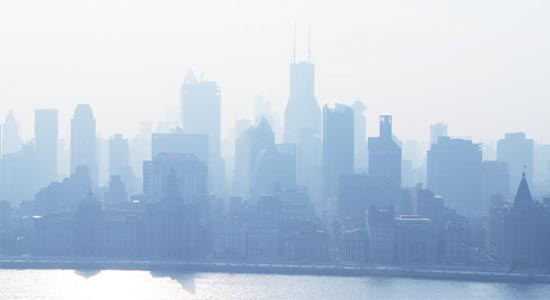
\includegraphics{PresentationPhotos/urbanPollution.jpg}

}

\caption{Urban smog in China}

\end{figure}%
\end{frame}

\begin{frame}{Discussion}
\phantomsection\label{discussion-1}
\begin{itemize}
\item
  The prior maps showed that factors are highly localized for most of
  our covariates
\item
  Expected exception for median income, which has a constant effect
  regardless of region
\end{itemize}
\end{frame}

\begin{frame}{Discussion}
\phantomsection\label{discussion-2}
\begin{itemize}
\item
  We observed localized impacts for African Americans, Hispanics, and
  Asians in different areas of the country
\item
  Limitation in race percentages presented by misreporting of medical
  records affecting minorities (Tabb et al.~2020). Shows that
  intervention is needed to combat racial health disparities that were
  caused by disparities in the healthcare system.
\end{itemize}
\end{frame}

\begin{frame}{Discussion}
\phantomsection\label{discussion-3}
\begin{itemize}
\item
  Looking at the Variance Inflation Factor (VIF) of our GWR model:

  \begin{table}[ht] \centering \begin{tabular}{rrrrrrr}   \hline 1 & 2 & 3 & 4 & 5 & 6 & 7 \\    \hline 183.22 & 196.12 & 7.24 & 2.56 & 1.15 & 2.44 & 2.62 \\    81.32 & 93.80 & 4.14 & 2.53 & 1.77 & 3.39 & 2.65 \\    302.16 & 313.78 & 16.89 & 4.06 & 1.27 & 2.42 & 2.09 \\    140.83 & 151.46 & 5.25 & 2.13 & 1.10 & 2.35 & 2.73 \\    131.77 & 128.39 & 8.33 & 2.67 & 1.07 & 2.34 & 2.32 \\    282.66 & 294.23 & 14.14 & 3.77 & 1.24 & 2.44 & 2.22 \\     \hline \end{tabular} \end{table}
\end{itemize}
\end{frame}

\begin{frame}{Discussion}
\phantomsection\label{discussion-4}
\end{frame}

\section{Conclusion}\label{conclusion}

\begin{frame}{Conclusion}
\phantomsection\label{conclusion-1}
\begin{itemize}
\item
  We have shown that a GWR model can be used to analyze the relationship
  between CVM and socioeconomic covariates.
\item
  The differing local significance that we detected highlights the need
  to identify region-speific interventions to curb the toll of CVD.
\end{itemize}
\end{frame}



\end{document}
